\chapter{Brockett-Bedingung für unteraktuiertes mechanisches System}
\label{Brockett_Bedingung_für_unteraktuiertes_mechanisches_System}

\section{Erläuterung zur Brockett-Bedingung}
\label{Erläuterung zur Brockett-Bedingung}
In Anbetracht von der mathematische Beschreibung und dem Beweis für Brockett-Bedingung ist zuerst die Erklärung einiger mathematischen Terme notwendig.    
\begin{description} 
	\item[Stetigkeit (engl.: continuous)]
	\cite[S.250]{grosche2003teubner}:~Es sei $a\subseteq M$. Die Funktion $f:M\subseteq\Reals\to\Reals$ ist genau dann im Punkt $a$ stetig, wenn es zu jeder reellen Zahl $\varepsilon>0$ eine reelle Zahl $\delta>0$ gibt, sodass
	$\left | f\left ( x \right )-f\left ( a \right ) \right |< \varepsilon$ für alle $x\subseteq M$ mit $\left | x-a \right |< \delta $ gilt.  
\end{description}
\vspace{-0.8em}
D.h. eine stetige Funktion erfüllt die Bedingung: wenn der Abstand zweier Elemente der Definitionsmenge infinitesimal ist, muss der Abstand ihrer entsprechenden Wertemenge auch infinitesimal sein.
\begin{description}
	\item[Stetige Differenzierbarkeit (engl.: continuously differentiable)]
	\cite[S.256]{rudin2009analysis}:~Eine differenzierbare Abbildung $\vect{f}:E\subset\Reals^{n}\to \Reals^{m}$ sei stetig differenzierbar in $E$, wenn ${\vect{f}}'$ eine stetige Abbildung von $E$ in $L\left ( \Reals^{n},\Reals^{m} \right )$ ist, wobei $E$ eine offene Menge und $L\left ( X,Y \right )$ Raum linearer Abbildungen ist.
	\item[Klasse $C^{k}$ (engl.: class $C^{k}$)]
	\cite[S.265]{grosche2003teubner}:~Eine Funktion auf einer offenen Umgebung des Punktes $p$ stetige Ableitungen bis zur Ordnung $k$ besitzt.
\end{description}
\vspace{-0.8em}
Basierend auf die obige Definition hat eine Funktion von Klasse $C^{1}$ die Ableitung 1. Ordnung, die auch stetig ist.
\begin{description}
	\item[Glatte Funktion (engl.: smooth function)]
	\cite[S.5]{tu2010introduction}:~Ein Synonym für $C^{\infty}$ ist ``Glatt''.
\end{description}
\vspace{-0.8em}
Eine glatte Funktion ist nämlich eine Funktion mit stetigen Ableitungen zur unendlichen Ordnung.
\begin{description}
	\item[Surjektiv (engl.: onto)]
	\cite[S.931]{grosche2003teubner}:~Gegeben sei die Abbildung $f:X \to Y$. Betrachtet die Gleichung $f\left ( x \right )=y$. Wenn die Gleichung für jedes $y\in Y$ eine Lösung $x\in X$ besitzt, d.h. $f\left ( X \right )=Y$, dann heißt $f$ genau dann \emph{surjektiv}.
\end{description}
\vspace{-0.8em}
Falls jedes Element $y$ der Wertemenge $Y$ kann erreicht werden, dann ist diese Abbildung surjektiv. 
\begin{description}
	\item[Homotopie (engl.: homotopy)]
	\cite[]{}(noch nicht geschrieben wird.)
\end{description}
\vspace{-0.8em}
\begin{description}
	\item[Häufungspunkt (engl.: limit point)]
	\cite[S.35]{rudin2009analysis}:~Ein Punkt $p$ ist ein \emph{Häufungspunkt} der Menge $E$, wenn in jeder Umgebung von $p$ ein Punkt $q\in E$ mit $q\neq p$ liegt.
	\item[Abgeschlossene Menge (engl.: closed set)]
	\cite[S.36]{rudin2009analysis}:~$E$ heißt abgeschlossen, wenn jeder Häufungspunkt von $E$ in $E$ liegt.
	\item[Beschränkte Menge (engl.: bounded set)]
	\cite[S.36]{rudin2009analysis}:~$E$ ist beschränkt, wenn eine reelle Zahl $M$ und ein Punkt $q\in X$ existieren, sodass der Abstand von $(p,q)$ kleiner als $M$ für alle $p\in E$ gilt. $X$ ist hier ein metrischer Raum, dessen Teilmenge $E$ ist.
	\item[Kompakte Menge (engl.: compact set)]
	\cite[S.45]{rudin2009analysis}:~(Satz, nicht Definition) Falls eine Menge $E$ in $\Reals^{k}$ abgeschlossen und beschränkt, dann ist sie kompakt.
\end{description}
\vspace{-0.8em}
Ein sehr einfaches Beispiel der kompakten Menge $E$ ist z.B. $\left [ 1,2 \right ]$ mit $1$ und $2$ jeweils dem linken und rechten Häufungspunkt. %Weil $1$ und $2$ gehört zur $E$ und der Abstand jeder beliebigen zwei Elementen in $E$ kleiner als z.B. $2$. Dagegen ist die Menge \left ( 1,2 \right ) nicht kompakt.  
\begin{description}
	\item[Niveaumenge (engl.: level set)]
	\cite[S.94]{tu2010introduction}:~Eine Niveaumenge einer Abbildung $f:N \to M$ ist die Submenge $f^{-1}\left ( c \right )= \left \{ p\in N \mid f\left ( p \right )= c\right \}$ für einige $c\in M$.
\end{description}
\vspace{-0.8em}
Also die Niveaumenge $f^{-1}\left ( c \right )$ besteht aus die Elemente der Definitionsmenge, deren Bildmenge eine Konstante $c$ ist.
\begin{description}
	\item[Distribution]
\end{description}
%\vspace{-0.8em}
\begin{description}
	\item[Lefschetz-fixed-point-formula]
\end{description}
\begin{description}
	\item[Lokale Lipschitzstetigkeit (engl.: locally Lipschitz continuity)]
	\cite[S.553]{bronstein2012taschenbuch}:~Lipschitz-Bedingung bezüglich $y$ ist die Forderung $\left | f\left ( x,t \right ) -f\left ( y,t \right )\right |\leq L\left | x-y \right |$ für alle $\left ( x,t \right )$ und $\left ( y,t \right )$. Inzwischen ist $L$ eine beliebige Konstante.
\end{description}
\vspace{-0.8em}
Das heißt, wenn die Ableitung der Funktion von $f$ beschränkt ist, erfordert sie Lipschitz-Bedingung. Die Lipschitzstetigkeit ist stärker als Stetigkeit.


%Lefschetz-fixed-point-formula, Poincare-Hopf Theorem %没写!!!!!!










Ein nichtlineares Zustandsraummodell lässt sich durch Gl. \ref{Zustandsraummodell} darstellen:
\begin{eqnarray}
\dot{\vect{x}}\left ( t \right )=\vect{f}\left (\vect{x}\left ( t \right ),u\left ( t \right )  \right ),~~~t\geq 0,~~~\vect{f}:\Reals^{n}\times\Reals^{m}\to\Reals^{n},~~~\vect{f}\left ({\vect{x}_{0}},0  \right )=\vect{0}
\label{Zustandsraummodell}
\end{eqnarray}
mit $\vect{x}$ dem Systemzustand, $\vect{f}$ der nichtlinearen Zustandsfunktion, $u$ der Eingangsgröße und $\vect{x}_{0}$ dem initialen Zustand. 

Jetzt stellt sich die Frage: gibt es die Möglichkeit, dass das obere nichtlineare System um die Ruhelage $\vect{x}=\vect{x}_{0}$ mit einer nichtlinearen Zustandsrückführung (nämlich hier $u$) asymptotisch stabilisierbar sein kann? Zum Antworten der Frage etabliert der amerikanische Mathematiker Roger W. Brockett das folgende berühmte Kriterium\cite{brockett1983asymptotic}:
\begin{theorem}[Brockett-Bedingung\cite{brockett1983asymptotic}]
	Betrachtet man das System $(\ref{Zustandsraummodell})$ mit $\vect{f}$ stetig differenzierbar in der Umgebung von $(\vect{x}_{0},0)$ ist. Angenommen, dass $(\vect{x}_{0},0)$ in $\Reals^{n}\times\Reals^{m}$ asymptotisch stabil unter einer stetigen differenzierbaren Rückführung $u$ ist, dann ist das Bild der Abbildung
	\begin{center}$\left ( \vect{x},u \right ) \mapsto f\left ( \vect{x},u \right )$\end{center}
	surjektiv zur offenen Menge, die 0 enthält.
\end{theorem}
Die obere notwendige Bedingung basiert auf eine \emph{zusätzliche} notwendige Bedingung: das linearisierte System enthält keines nicht steuerbares Moduls, dessen Eigenwerte in  der rechte Halbebene liegen. Wenn $(x_{0},0)$ asymptotisch stabil ist, hat das linearisierte System nur steuerbare Module (mit oder ohne Eigenwerte in der rechte Halbebene) oder nicht steuerbare Module mit stabilen Eigenwerte. Mit anderen Worten muss instabile Module steuerbar oder nicht steuerbare Module stabil sein.

Ein leicht verwirrender Punkt dieses Kriterium liegt in die Bedingungen von $\vect{f}$ und $u$ in Gl. \ref{Zustandsraummodell}. Nach der Beschreibung des Theorems sind beide $\vect{f}$ und $u$ \emph{stetig differenzierbar}, und in dem Beweis zitiert Brockett eine stetig differenzierbare Lyapunov Funktion, die aber im Original \emph{glatt} ist. (siehe \cite[S.186]{brockett1983asymptotic} und \cite[S.324]{wilson1967structure}.) In anderen Literaturen sind auch unterschiedliche Annahmen ermöglicht: \cite{coron2007control} und \cite{orsi2003necessary} setzen $\vect{f}$ und $u$ \emph{stetig und zeitinvariant} als bekannt voraus, während in \cite{stern2002brockett} und \cite{colonius2012nichtlineare} bringen die Autoren strengeren Bedingung vor: \emph{lokal lipschitz}. Im Buch vom argentinischen Mathematiker Eduardo D. Sontag \cite{sontag2013mathematical} werden die Bedingung von $\vect{f}$ und $u$ gleich wie Brockett ($C^{1}$). Eine noch strengere Voraussetzung werde von G. Oriolo und Y. Nakamura in \cite{oriolo1991control} aufgestellt, dass $\vect{f}$ \emph{stetig differenzierbar} und $u$ \emph{glatt} sein muss.

Zurück auf Brocketts Beweis?????????????????????????

\begin{proof}[\textbf{Skizze des Beweises} (\cite{brockett1983asymptotic},\cite{liberzon2012switching})]~Falls die Ruhelage $(\vect{x}_{0},0)$ asymptotisch stabil ist, existiert es nach \cite{wilson1967structure} eine glatte Lyapunov Funktion $V$, die eine sphärischer homotopy Niveaumenge $V^{-1}(c)$ ($c$ eine kleine Konstante) hat. Wegen der Kompaktheit von $V^{-1}(c)$ ist die Richtung von $f(\vect{x},u)$ \emph{in} der Menge $R:= \left \{ \vect{x}:V\left (\vect{x}  \right )\leq c \right \}$. Es existiert auch $\xi \in \Reals^{n}$ mit $\left \| \xi \right \|$ genügend klein, dass $f(\vect{x},u)-\xi$ auch \emph{in} $R$ zeigt. Durch die Anwendung des Fixpunktsatz gilt es $f(\vect{x},u)-\xi=0$ (oder $f(\vect{x},u)=\xi$) für einige $\vect{x}$ in $R$. Weil $\left \| \xi \right \|$ beliebig und sehr klein ist, bedeutet die obige Funktion, dass $f$ lösbar in beliebiger Umgebung von 0 ist.
\end{proof} %\qed  

\section{Ausgang: Doppelintegrator}
\label{Doppelintegrator}
Doppelintegrator ist ein erfüllendes Brockett-Bedingung Beispiel. Die asymptotische Stabilität kann man mithilfe des Paket \emph{Pytrajectory} überprüfen. Das lineariserte affine System davon lautet:
\begin{eqnarray}
\dot{\vect{x}} = \begin{bmatrix}
0 & 1\\ 
0 & 0
\end{bmatrix}\vect{x} + \begin{bmatrix}
0\\1 
\end{bmatrix}u
\label{eq:doppel_Sytemzustand}
\end{eqnarray}
mit der Steuerbarkeitsmatrix $Q_{s} = \begin{bmatrix}
0 & 1\\ 
1 & 0
\end{bmatrix}$ und $rang(Q_{s})=2$. Das System ist vollständig steuerbar. Die zusätzliche Bedingung erfüllt.

Jetzt wird die Brockett-Bedingung überprüft. Setzt man voraus, dass $\vect{\epsilon}$ in der offenen Menge von $0$ liegt, dann ist 
\begin{eqnarray}
\vect{\epsilon}  = \begin{bmatrix}
\epsilon _{1}\\ \epsilon_{2}
\end{bmatrix} = 
\begin{bmatrix}
x_{2\epsilon }\\ u_{\epsilon }
\end{bmatrix}
\label{eq:doppel_Brockett}
\end{eqnarray}
Gl. \ref{eq:doppel_Brockett} kann jeden Wert in der Umgebung von $\vect{0}$ ohne Ausnahme erreichen. Dann ist die Brockett-Bedingung automatisch erfüllt. $\vect{x_{0}} = (x_{belibig}, 0)$ ist eine asymptotisch stabile Ruhelage.

\section{Unteraktuiertes mechanisches System}
\label{Unteraktuiertes_mechanisches_System}

\section{Ausgang: Zwei-Gelenke-Manipulator}
\label{Ausgang_Zwei_Gelenke_Manipulator}
\begin{figure}
	\centering
	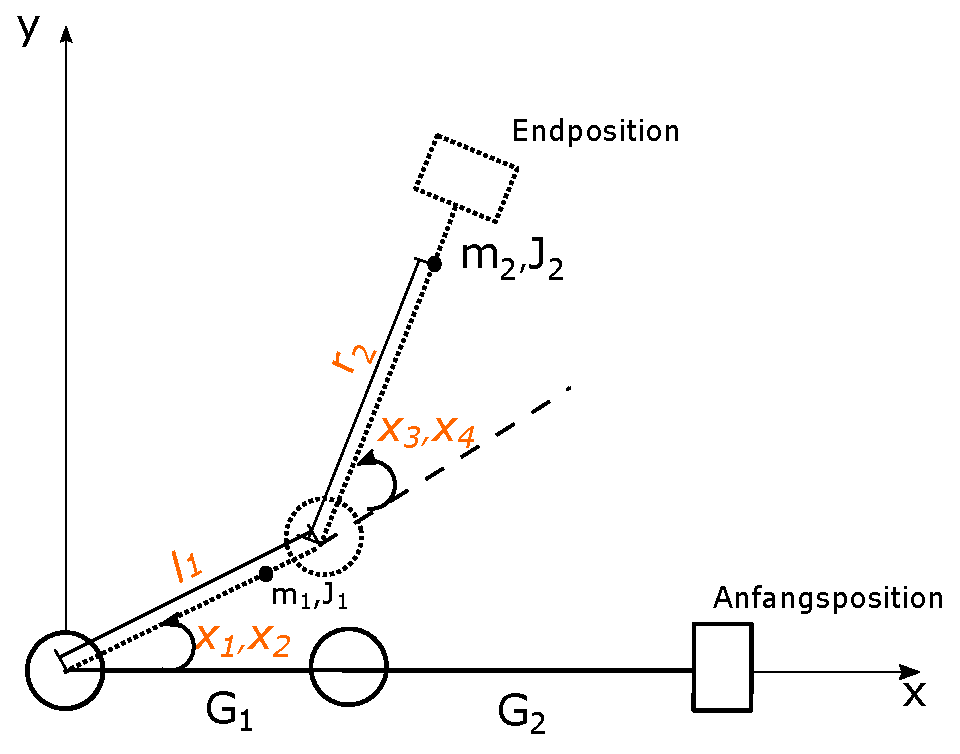
\includegraphics[width=8cm]{bild/modul/Unteraktuiertes-System.eps}
	\caption{Gütefunktion von k: $x_{min}=0$, $x_{max}=10$}
	\label{fig:Gütefunktion_von_k}
\end{figure}